\documentclass{article}

\usepackage[utf8]{inputenc}

% Packages
\usepackage{amsmath,amssymb}
\usepackage{bm}% boldmath
\usepackage{listings} % Code block (source code) \begin{lstlisting} 
\usepackage{natbib}
\usepackage{graphicx}
\usepackage{lmodern}
\usepackage[usenames,dvipsnames,svgnames,table]{xcolor}
\usepackage[textwidth=16cm,textheight=23cm]{geometry}

%\usepackage{inconsolata} % New monospace font

% URL
\usepackage{url}
\usepackage[colorlinks=true, a4paper=true, pdfstartview=FitV, linkcolor=blue, citecolor=blue, urlcolor=blue]{hyperref}

% Figures
\usepackage[font=small, labelfont=bf]{caption}
\usepackage{subfig} % Subfigures. Uses \subfloat[captions text]{figure}

% Tables
\usepackage{booktabs}   % Allows the use of \toprule, \midrule and \bottomrule in tables for horizontal lines
\newcommand{\ra}[1]{\renewcommand{\arraystretch}{#1}} % spaces in tables

% Itemize
\usepackage{enumitem}

% Commands
%\newcommand{\code}[1]{\texttt{#1}} % \code{inline code}
\newcommand{\code}[1]{{\small\ttfamily #1}} % \code{inline code}
\newcommand{\expval}[1]{\langle #1 \rangle} %
\renewcommand{\theequation}{\arabic{section}.\arabic{equation}} % Book format equation
\renewcommand{\thefigure}{\arabic{section}.\arabic{figure}} % Book format figure
\renewcommand{\vec}[1]{{\bf #1}} % Lars likes this better than arrow

% Set page attribution
\setlength{\parindent}{0pt}


% PSTRICKS
\usepackage{pstricks,pst-node,pst-tree} % includes graph additions
\usepackage{pst-pdf} % Compiles the pictures
\usepackage{pst-node}
\usepackage{pst-plot}
\usepackage{pst-3dplot}
%\usepackage{pstricks-add,babel}




\lstset{
language=Python,                        % Code langugage
commentstyle=\color{gray},              % Comments font
basicstyle=\small\ttfamily,             % Code font, Examples: \footnotesize, \ttfamily
keywordstyle=\bfseries\color{blue},
stringstyle=\color{orange},
numbers=left,                           % Line nums position
numberstyle=\tiny,                      % Line-numbers fonts
stepnumber=1,                           % Step between two line-numbers
numbersep=5pt,                          % How far are line-numbers from code
frame=none,                             % A frame around the code
tabsize=4,                              % Default tab size
captionpos=b,                           % Caption-position = bottom
breaklines=true,                        % Automatic line breaking?
breakatwhitespace=false,                % Automatic breaks only at whitespace?
showspaces=false,                       % Dont make spaces visible
showstringspaces=false,                 % Dont make spaces visible in strings
showtabs=false,                         % Dont make tabls visible
belowskip=8pt,
morekeywords={range, xrange},
% backgroundcolor=\color{yellow}
% emph={[2]root,base}
% morekeywords={one,two,three,four,five,six,seven,eight,
}


%commentstyle=\color{gray},              % Comments font
%basicstyle=\small,                      % Code font, Examples: \footnotesize, \ttfamily



%basicstyle=\footnotesize\ttfamily,
%keywordstyle=\bfseries\color{green!40!black},
%commentstyle=\itshape\color{purple!40!black},
%identifierstyle=\color{blue},
%stringstyle=\color{orange},





\usepackage{siunitx}

% ***************************************************
% HEADER INFORMATION

\title{Exercise 5}
\author{Molecular Statistics, Week 5}
\date{}

% ***************************************************

\begin{document}


% ***************************************************
% BEGIN DOCUMENT
% ***************************************************

\maketitle

\section{Introduction}

Often it will be necessary to data-mine, manipulate and visualize data obtained manually from experiments or from other software.
Python is great for this and the goals of this exercise is:

\begin{enumerate}
    \item Use Python to load/read data

    \item Use Numpy to manipulate data

    \item Use matplotlib to illustrate data

    \item Use string manipulation for tables

\end{enumerate}


Note to remember.
If you sit with some data and you do not know how to plot the specific plot, then take a look at
\href{http://matplotlib.org/1.3.1/gallery.html}{matplotlib.org/1.3.1/gallery.html} for inspiration.



\subsection{Changing the look of matplotlib}
%TODO change?
You can change pretty much anything in a matplotlib plot using the \code{rc} function.
A small header file to override most of the default stuff in matplotlib to make it look more professional can be found here
\href{https://github.com/charnley/matplotlib-header}{github.com/charnley/matplotlib-header}.
Here is a before / after example.

\begin{figure}[htb]
  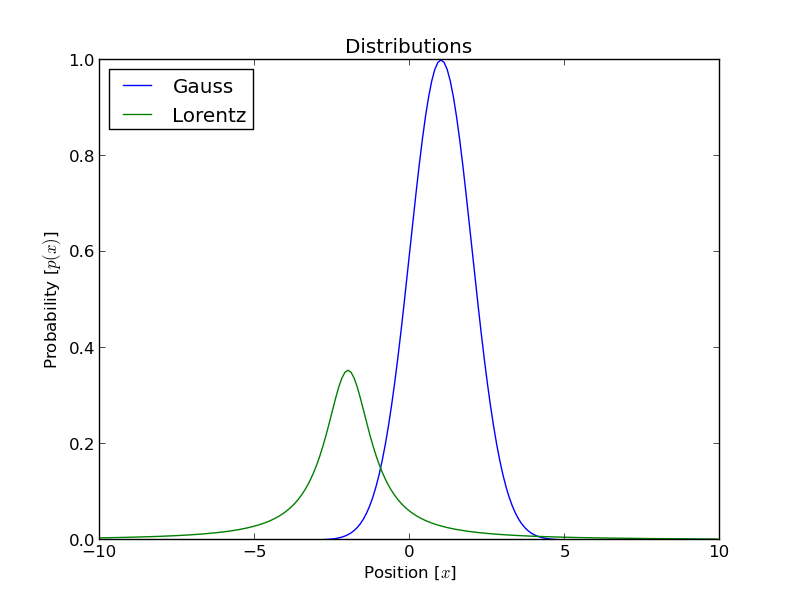
\includegraphics[width=0.5\textwidth]{images/figure_xy_before.png}
  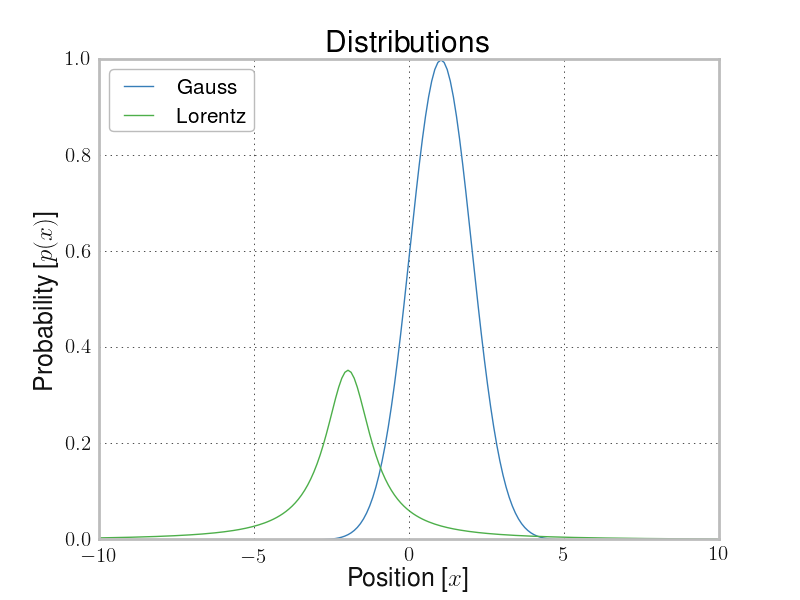
\includegraphics[width=0.5\textwidth]{images/figure_xy_after.png}
\end{figure}




\section{Exercises}

Todays exercises will each be based on different sets of data which requires different plot representation.
You will be given different data files to load/read in Python.
Try to use Google to answer questions you might have, as not all details you need are included in the exercises.

\newpage
\subsection{Energy of a covalent bond during stretching}

This data represents what will happen to the overall energy if you move a hydrogen, in a water-dimer, away from it's global minimum.
This is calculated with 4 different methods and stored in corresponding data files.
The data is structured like this:

\begin{lstlisting}
    -0.30   0.000000000   1.094813771   -0.789196930   -152.5782121321
\end{lstlisting}

The first column is the displacement of the hydrogen in \AA ngstrom. The next three are the dipole-moment (which we are not using) and the last is the total energy in Hartree.\\

Your job is to see if the four energy models, B3LYP, CCSD(t), CCSD(t)-F12 and MP2 describes a similar energy surface or not.\\

{\bf Exercise Hint:}
If you have no idea where to start use the following code as inspiration:

\begin{lstlisting}
f = open('method.dat', 'r')
for line in f:
    print line

\end{lstlisting}

Also look up what the command \code{continue} does in a for-loop and what the method \code{.split()} does with a string. %why continue?

\begin{enumerate}
    % Haven't had numpy yet
    \item Load all the energies into a list and a corresponding list for displacement,
          for each method.
          Plot the data in the same plot.

    \item Remember to add labels for axis and methods.

    \item Convert the energy to kcal/mol.
          Plot the result.

    \item Usually when computing quantum chemical energies, we are not interested in absolute values.
          Plot the relative change in energy away from the displacement = 0.0.

\end{enumerate}

\newpage
\subsection{Simulated UV-Vis spectra}
This data represent energy and oscillator strength of allowed transitions in a boron subphlatocyanine molecule. The data is structured like this:
\begin{lstlisting}
    2.4918 0.4790
\end{lstlisting}
where the first column is the transition energy in electron volt (eV), the second is the oscillator strength of the transition (unit less).\\

Since the spectrum in most cases will be of more than one excitation the collected spectrum must be investigated for all wavelengths of interest, say form $200\si{nm}$ to $700\si{nm}$ and then summed over all the oscillator strengths found.
\begin{equation}
\epsilon(\lambda)=\sum_{j=1}^n \epsilon_j(\lambda)=\sum_{j=1}^n  \underbrace{\frac{\text{N}_A\si{e^2}}{2\ln(10) \text{m}_e \epsilon_0\si{c^2}} \sqrt{\frac{\ln(2)}{\pi}}}_\text{k x 10} \frac{f^j}{\sigma} \exp{\Bigg(-4 \ln(2) \left[\frac{\left(\frac{1}{\lambda}-\frac{1}{\lambda_{if}^j}\right)}{\sigma\cdot 10^{-7}}\right]^2}\Bigg) \si{M^{-1}cm^{-1}} \label{eq_uv_vis}
\end{equation}

where $f^j$ and $\lambda_{if}^j$ are the oscillator strength and wavelength related to the $\text{j}^{th}$ transition and $n$ is the total number of transitions in the dataset. The other constants are:

\begin{center}
\begin{tabular}{|c|c|}
\hline 
$N_A$ & Avogadros Number \\ 
\hline 
$e$ & Elemental charge \\ 
\hline 
$m_e$ & Electron mass \\ 
\hline 
$\epsilon$ & Vacuum permittivity \\ 
\hline 
$c$ & Speed of light \\ 
\hline 
\end{tabular} 
\end{center}



$\sigma$ is the full width half maximum of the Gaussian function used to convolute the UV-vis spectra. It defines the width of the absorption peaks. In this example we will use $\sigma = 3226 \si{cm^{-1}}$.
\begin{enumerate}
\item Find the values in Si-units of all the natural constants needed to calculate the UV-vis spectra and define them as variables. e.g. \\

\item Define a constant $k=\frac{\text{N}_A\si{e^2}}{2\ln(10) \text{m}_e \si{c^2}  \epsilon_0}\sqrt{\frac{\ln(2)}{\pi}}\cdot 10^{-1} \frac{\si{L}}{\si{mol}}\si{cm^{-2}}$ and use all the variables you just defined to calculate the value of $k$. Print the value of $k$. If you have done this correctly you should find
$k=217512853.406$
\end{enumerate}

Now we are ready to calculate the UV-Vis spectra. 
\begin{enumerate}[resume]
\item Load all the transition energies from the file \code{data1\_uv\_vis.dat} into a list called \code{transition\_list}, and oscillator strengths into a list called \code{osillator\_list}
\item Make a third list \code{wavelengths=[]} starting at 200 and ending at 700 with length 500 - these are all the points at which you want to calculated the total absorption, given as $\lambda$ in \eqref{eq_uv_vis}. \textit{Hint} use \code{np.linespace()}
\end{enumerate}

In order to plot the UV-Vis spectra via \eqref{eq_uv_vis}, the transition energies must be converted to nano-meters instead.

\begin{enumerate}[resume]
\item Convert all transition energies from eV to nm.
\item Loop over all transitions and calculate the total intensity first at 200nm, then at 350nm and finally at 500nm

\item Make an outer loop to calculate the total absorption intensity at all wavelengths from 200nm to 700nm \label{outerloop}
\item Plot the result - remember to add legend, labels and title to the plot with units on the axis, where the y-axis should include the symbol $\varepsilon$.

\end{enumerate}

Next step is to plot two UV-Vis spectra in one. In order to do this you  must first define a function that takes as input transition energies in nm, oscillator strength and the wavelengths for which the spectra is to be plotted. The function should return total absorption intensity

\begin{enumerate}[resume]
\item Define a function that calculates the total absorption at each $\lambda$ based on the loop from exercise \ref{outerloop}
\end{enumerate}


\newpage
\subsection{Binding free energies}

This data represents a theoretical thermodynamic study of host-ligand binding energies.
The data is from Gilson {\em et al.}\footnote{Hari S. Muddana and Michael K. Gilson, dx.doi.org/10.1021/ct3002738 | J. Chem. Theory Comput. 2012, 8, 2023-2033}
The system in question is the Cucurbit7uril (CB7) host molecule with different organic ligands inside it.
Calculations of the binding energy ($\Delta G^\circ$) have been done based on a semi-empirical method called PM6-DH+.
The result of these calculations are stored in \code{calculated\_new.csv} and has the following structure:

\begin{lstlisting}
1 -139.8 130.3 -0.0318791946309
\end{lstlisting}

The columns are respectively ID, change in enthalpy ($\Delta U$) [kcal/mol], change in solvent energy ($\Delta W$) [kcal/mol] and lastly change in entropy ($\Delta S^\circ$) [(kcal/mol)/Kelvin].
The binding energy is then calculated with the following formula:

\begin{align}
    \Delta G^\circ = \Delta U - T \Delta S^\circ + \Delta W + \delta
\end{align}

where $\delta$ is an empirical parameter set to $-5.83$ kcal/mol and $T$ is the temperature of 298.0 Kelvin.\\

Similarly the \code{experimental.csv} contains the experimental binding energies with the following data structure:

\begin{lstlisting}
1, -5.3
\end{lstlisting}

where the columns are ID and binding energy in kcal/mol respectively.

\begin{enumerate}

    \item Load the data into corresponding lists and calculate the theoretical binding energies using the above equation.

    \item Plot the experimental vs calculated energies.

    \item Add a fixed $x = y$ line to the plot.
        Fix the limits of the x and y axis to match each other, to better visualize how correct the calculated $\Delta G^\circ$ are.

    \item Add two fixed dotted lines representing +/- 2 kcal/mol experimental uncertainty. 

    \item Calculate the Pearson Correlation factor $r$ and corresponding $p$ value.
        Does the calculated energies correlate with the experimental values?
        {\bf Hint:} Search for the \code{scipy} module for a nice Pearson function.

    \item Calculate the Root-mean-square deviation (RMSD) between the experimental and calculated binding energies.
    \begin{align}
        \mathrm{RMSD} = \sqrt{\frac{\sum_i^N (x_{\mathrm{exp}}-x_{\mathrm{cal}})^2 }{n}}
    \end{align}

    \item As you might have noticed, there are two outliers with over 4.5 kcal deviation from the experimental value.
        Use \code{plt} to highlight which of the ligands - by their ID-number these are ,in the plot.
        {\bf Hint:} Use the method \code{plt.text()} as described in the matplotlib guide / internet.

\end{enumerate}

%Det her er helt uforståeligt. Kan ikke overskue det.

If you are using \LaTeX, you will want to print out data directly as a \LaTeX table.
This can be done with the method \code{.format()}.


\begin{enumerate}[resume]

    \item Print the ligand id, experimental and calculated energy out as a \LaTeX table

\end{enumerate}




\newpage
\iffalse
\subsection{Random precision errors in assigned chemical shifts}

When assigning measured chemical shifts of a protein to their respective amino-acids you will have to match the chemical shift measured by one experiment with another.
Due to experimental error these values are not exactly the same, even though they should be in theory.
Because of this it can be difficult to be sure that the two matched chemical shifts actually origin from the same amino-acid.
To avoid making assignment errors it is thus informative to know how well the measured chemical shifts 'should' match.\\

The file \code{chemical\_shift\_errors.txt} obtained from the course website contains all differences (or errors) in assigned chemical shifts of all amide protons for a single protein in a single column format.


\begin{enumerate}

    \item Load the file containing the data and store it a variable.

    \item Plot a histogram of the data using Matplotlib.

\end{enumerate}

When plotting a histogram you can select the number of bins to present the data with by giving the argument \code{bins=10}. (10 is the default value in Matplotlib).
%If you try changing the number of bins you can severely affect how the data 'looks', especially if your number of datapoints are relatively low.
%% put this in since all this shouldn't take long for the students to do.
%The Freedman-Diaconis Rule can be used to select the number of bins automatically.
%The following code takes as argument the data and returns the optimal number of bins according to the Freedman-Diaconis Rule.
%
%\begin{lstlisting}
%def bins(data):
%    data.sort()
%    n=len(data)
%    width = 2*(data[3*n/4]-data[n/4])*n**(-1./3)
%    return int((data[-1]-data[0])/width)
%\end{lstlisting}

%\begin{enumerate}[resume]
%
%    \item Plot the histogram again using the Freedman-Diaconis Rule to select number of bins.
%
%\end{enumerate}

If these errors are completely random, they should approximately follow a normal distribution (also known as a Gaussian distribution).
We can use the module \code{scipy.stats} to fit a distribution to a dataset.
Import this in your program as follows:

\begin{lstlisting}
import scipy.stats as ss
\end{lstlisting}

We will begin by fitting a normal distribution to our data.
The command \code{ss.norm.fit(data)} returns the mean and standard deviation that best describes the data.
To draw this curve we will need a set of $x$ and $y$-values that cover our data range.

\begin{enumerate}[resume]

    \item Use \code{np.arange()} together with the \code{max()} and \code{min()} functions to generate $x$-values that range from the lowest data point to the highest in steps of \code{1e{-3}}. Store these in a variable called \code{x}.

\end{enumerate}

The function \code{ss.norm.pdf(x, param\_1, param\_2)} returns the probability densities for a normal distribution for all values of \code{x}.
\code{param\_1} and \code{param\_2} are the mean and standard deviation you obtained from the fit.

%Fitting more complicated distributions will return more than two parameters.
%To avoid having to adjust the number of arguments for each distribution you look at, the following works for every distribution in the \code{scipy.stats} package:

\begin{lstlisting}
param_1, param_2 = ss.norm.fit(data)
y = ss.norm.pdf(x, param_1, param_2)
\end{lstlisting}


\begin{enumerate}[resume]

    \item Fit a normal distribution to your data.

    \item Try to plot the fitted distribution together with the histogram. \emph{Hint!} Use \code{normed=1} as argument to your histogram.

    %\item Try fitting other popular distributions such as the Cauchy/Lorenz distribution \code{ss.cauchy} or the Student's t-distribution \code{ss.t}.

\end{enumerate}


\newpage
\subsection{Protein structure determination}

Not all protein structures can easily be determined experimentally.
These kinds of proteins will often have their structure determined by simulation where a force-field is used to describe how the atoms interact with each other.
If a good force-field is used, the correct (also called native) structure should correspond to the lowest energy of the force-field.
When developing new force-fields you want to see how well the energy correlate with the deviation from the native structure.\\

The file \code{rmsd\_energy\_unfolded.txt} obtained from the course website, contains the energies, in units of $kcal/(mol\cdot RT)$ at $300K$, of several proposed structures as well as the atomic root mean square deviation (rmsd) in Å from the native structure.
You will never get an rmsd of zero for structures proposed by simulation, since the force-field will never fully describe all interactions correctly, however rmsds under 3-5 Å is usually considered accurate.\\

\emph{Note:} The first column contain the rmsds and the second one the energies.


\begin{enumerate}[start=1]

    \item Load the datafile in Python and put the rmsds in one list, and the energies in another.

    \item Plot the rmsds vs. energies using small black dots. Does the force-field used seem to be good in this case?

\end{enumerate}

Since the local energy minimum is not exactly at 0 Å it can be hard to know if you have achieved the correct structure and the non-zero rmsd stems from the force-field, or if an incorrect structure is found.
To test this a second simulation is usually run starting from the native structure to what the structure relaxes to with the given force-field.


\begin{enumerate}[resume]

    \item Download and load the file \code{rmsd\_energy\_native.txt}.

    \item Plot this together with the data from before, using a red colour. \emph{Note!} Change the border colour of the dots to red as well.

    \item Based on this second simulation, would you say that the force-field performs well?

\end{enumerate}

\fi
\newpage
\subsection{3D Gaussian}

Instead of plotting data in 3 dimensions (which is also possible with matplotlib), we can use the \code{plt.imshow()} function that shows the extra plane with colors.

To illustrate this method we will be using a two-dimensional independent Gaussian function, which is defined as;

\begin{align}
  f(x,y) = A \exp \left ( - \left ( \frac{(x - x_o)^2}{2\sigma_x^2} + \frac{(y - y_o)^2}{2\sigma_y^2} \right ) \right )
\end{align}

where we set $x_o = y_o = 0.0$, $A = 1.0$, $\sigma_x = 1.0$ and $\sigma_y = 2.0$.\\


\begin{enumerate}

    \item Define the Gaussian function, and the arrays for the $x$ and $y$ values.

    \item Create an array \code{Z} with the Gaussian function values.

\end{enumerate}

Now we want to illustrate the function using the \code{plt.imshow()} function, which is used like this:

\begin{lstlisting}
extent = [X[0], X[-1], Y[0], Y[-1]]      # extent defines the edges of the plot

im = plt.imshow(Z,
                interpolation='nearest', # Disable smoothing of the data.
                extent=extent,           # Use the defined axis/edges
                origin='lower',          # Corrects the origin
                cmap='gray')             # cmap defines what colormap to be used
\end{lstlisting}

The \code{origin='lower'} parameter is needed to make sure the data starts at the correct position.
Set \code{Z[-1][-1] = 1.0} and remove the parameter to see what it does.

\begin{enumerate}[resume]

    \item Plot the Gaussian array using the above code.

    \item Find a suitable colormap

\end{enumerate}

You can add a colorbar by using the colorbar function.

\begin{lstlisting}
cbar = plt.colorbar(im)
cbar.set_label('Text here', rotation=270)
\end{lstlisting}

Notice the rotation parameter. It is there to make it easier to read the label.

\begin{enumerate}[resume]

    \item Add a colorbar to the plot, with and without the rotation parameter

\end{enumerate}

Sometimes it is necessary to only use a part of the data only.

\begin{enumerate}[resume]

    \item Plot the data at $x$ = 1.0 for the full range of $y$.

\end{enumerate}


% ***************************************************
% END DOCUMENT
% ***************************************************

\end{document}
